% --------------------------------------------------------------------------- %
% --------------------------------------------------------------------------- %
\section{Lost Lepton Estimate}
\label{sec:lostlep}

The lost lepton background is predicted by taking the yield of single lepton events in similar kinematic regions, measuring the ratio of events where the lepton is lost to those where it is found, and extrapolating into the lost lepton regime. The control region for the lost lepton estimate is described in detail in section \ref{subsec:leptonCR}, and is comprised of events in data with the same signal triggers and preselection, with the exception of an inverted lepton veto and an additional requirement on lepton $M_{\mathrm{T}}$ (to reduce signal contamination). 

\subsection{Background Prediction}
\label{subsec:lostlepPrediction}

The estimate in a given signal region is obtained from a control region using transfer factors as described in equation \ref{eq:lostlepEstimate}, where $N_{\mathrm{1L}}^{\mathrm{CR}}$ is the number of events in the corresponding CR, $R_{\mathrm{MC}}^{0l/1l}$ is the ratio of zero-lepton to one-lepton events derived from simulation, and $k(\mttwomath)$ is the transfer factor into bins of \mttwo in a given topological region. The ratio $R_{\mathrm{MC}}^{0l/1l}$ is measured in Monte Carlo after normalizing the yield to data in each CR and correcting for differences in lepton efficiency between data and simulation, and also factors in lepton acceptance, efficiency of reconstruction and identification, as well as contributions from W bosons decaying through $\tau$ leptons to a hadronic final state. The \mttwo transfer factor $k(\mttwomath)$ is taken from data where statistics permit, and uses information from simulation to project events into bins of \mttwo in the low-statistics regime.
\begin{equation}
	N_{\mathrm{LL}}^{\mathrm{SR}}(\HT,N_\mathrm{j},N_\mathrm{b},\mttwomath) = N_{\mathrm{1L}}^{\mathrm{CR}}(\HT,N_\mathrm{j},N_\mathrm{b},\mttwomath) \cdot R_{\mathrm{MC}}^{0l/1l}(\HT,N_\mathrm{j},N_\mathrm{b},\mttwomath) \cdot k(\mttwomath)
	\label{eq:lostlepEstimate}
\end{equation}

To reduce the dependence of the estimate on the \mttwo shape modeling in simulation, the transfer factor $k(\mttwomath)$ uses a combination of data and simulation information. In each topological region, the greatest \mttwo bin is iteratively combined with the next-greatest bin until the total expected SM background yield in simulation is at least 50 events. These combined bins together form the CR for a range of \mttwo values, where the fraction of events falling in a particular \mttwo bin, $k(\mttwomath)$, is determined from simulation. In all the other \mttwo bins in the topological region, statistics are sufficient for a direct measurement in data and $k(\mttwomath)=1$. The extrapolation point for each topological region can be found in table \ref{tbl:lostlepHybridPoint}. The shape modeling in simulation is verified in data by selecting an inclusive sample enriched in either W boson or \ttbar production (using the number of b-tags in the event), and predicting the \mttwo distribution using simulation after normalizing simulation yield to data and summing all the control regions together, as seen in figure \ref{fig:lostlepHybrid}.
\begin{table}
	\centering
	\caption{The last \mttwo bin and the \mttwo extrapolation point for each topological region, beyond which shape data from simulation is used to extrapolate the lost lepton estimate into \mttwo bins.}
	\footnotesize
	\renewcommand{\arraystretch}{0.4}
	\begin{tabular}{c|c|c|c|c}
\hline \hline
\multicolumn{3}{c|}{Control Region} & Extrapolation Point & Last $\text{M}_{T2}$ bin  \\
$\text{H}_{T}$ [GeV] & $\text{N}_{j}$ & $\text{N}_{b}$ & $\text{M}_{T2}$ [GeV] & $\text{M}_{T2}$ [GeV]\\
\hline
$[250,450]$ &2-3&0& $>$ 300& $>$ 400\\
$[250,450]$ &2-3&1& $>$ 300& $>$ 400\\
$[250,450]$ &2-3&2& $>$ 300& $>$ 400\\
$[250,450]$ &4+&0& $>$ 300& $>$ 400\\
$[250,450]$ &4+&1& $>$ 300& $>$ 400\\
$[250,450]$ &4+&2& $>$ 200& $>$ 400\\
$[250,450]$ &2-3&3+& $>$ 200& $>$ 400\\
$[450,575]$ &2-3&0& $>$ 400& $>$ 500\\
$[450,575]$ &2-3&1& $>$ 300& $>$ 500\\
$[450,575]$ &2-3&2& $>$ 200& $>$ 500\\
$[450,575]$ &4-6&0& $>$ 400& $>$ 500\\
$[450,575]$ &4-6&1& $>$ 300& $>$ 500\\
$[450,575]$ &4-6&2& $>$ 300& $>$ 500\\
$[450,575]$ &7+&0& $>$ 200& $>$ 400\\
$[450,575]$ &7+&1-2& $>$ 200& $>$ 400\\
$[450,575]$ &2-6&3+& $>$ 200& $>$ 500\\
$[575,1000]$ &2-3&0& $>$ 600& $>$ 800\\
$[575,1000]$ &2-3&1& $>$ 400& $>$ 800\\
$[575,1000]$ &2-3&2& $>$ 200& $>$ 800\\
$[575,1000]$ &4-6&0& $>$ 400& $>$ 800\\
$[575,1000]$ &4-6&1& $>$ 400& $>$ 800\\
$[575,1000]$ &4-6&2& $>$ 400& $>$ 800\\
$[575,1000]$ &7+&0& $>$ 300& $>$ 800\\
$[575,1000]$ &7+&1-2& $>$ 300& $>$ 600\\
$[575,1000]$ &2-6&3+& $>$ 200& $>$ 600\\
$[1000,1500]$ &2-3&0& $>$ 400& $>$ 1200\\
$[1000,1500]$ &2-3&1& $>$ 200& $>$ 1200\\
$[1000,1500]$ &2-3&2& $>$ 200& $>$ 1000\\
$[1000,1500]$ &4-6&0& $>$ 400& $>$ 1200\\
$[1000,1500]$ &4-6&1& $>$ 400& $>$ 1200\\
$[1000,1500]$ &4-6&2& $>$ 200& $>$ 1000\\
$[1000,1500]$ &7+&0& $>$ 200& $>$ 1000\\
$[1000,1500]$ &7+&1-2& $>$ 200& $>$ 800\\
$[1000,1500]$ &2-6&3+& $>$ 200& $>$ 600\\
$[1500,\infty]$ &2-3&0& $>$ 200& $>$ 1400\\
$[1500,\infty]$ &2-3&1& $>$ 200& $>$ 1000\\
$[1500,\infty]$ &2-3&2& $>$ 200& $>$ 400\\
$[1500,\infty]$ &4-6&0& $>$ 400& $>$ 1400\\
$[1500,\infty]$ &4-6&1& $>$ 200& $>$ 1400\\
$[1500,\infty]$ &4-6&2& $>$ 200& $>$ 800\\
$[1500,\infty]$ &7+&0& $>$ 200& $>$ 1000\\
$[1500,\infty]$ &7+&1-2& $>$ 200& $>$ 800\\
$[1500,\infty]$ &2-6&3+& $>$ 200& $>$ 600\\
\hline \hline
	\end{tabular}
	\label{tbl:lostlepHybridPoint}
\end{table}
\begin{figure}
	\centering
	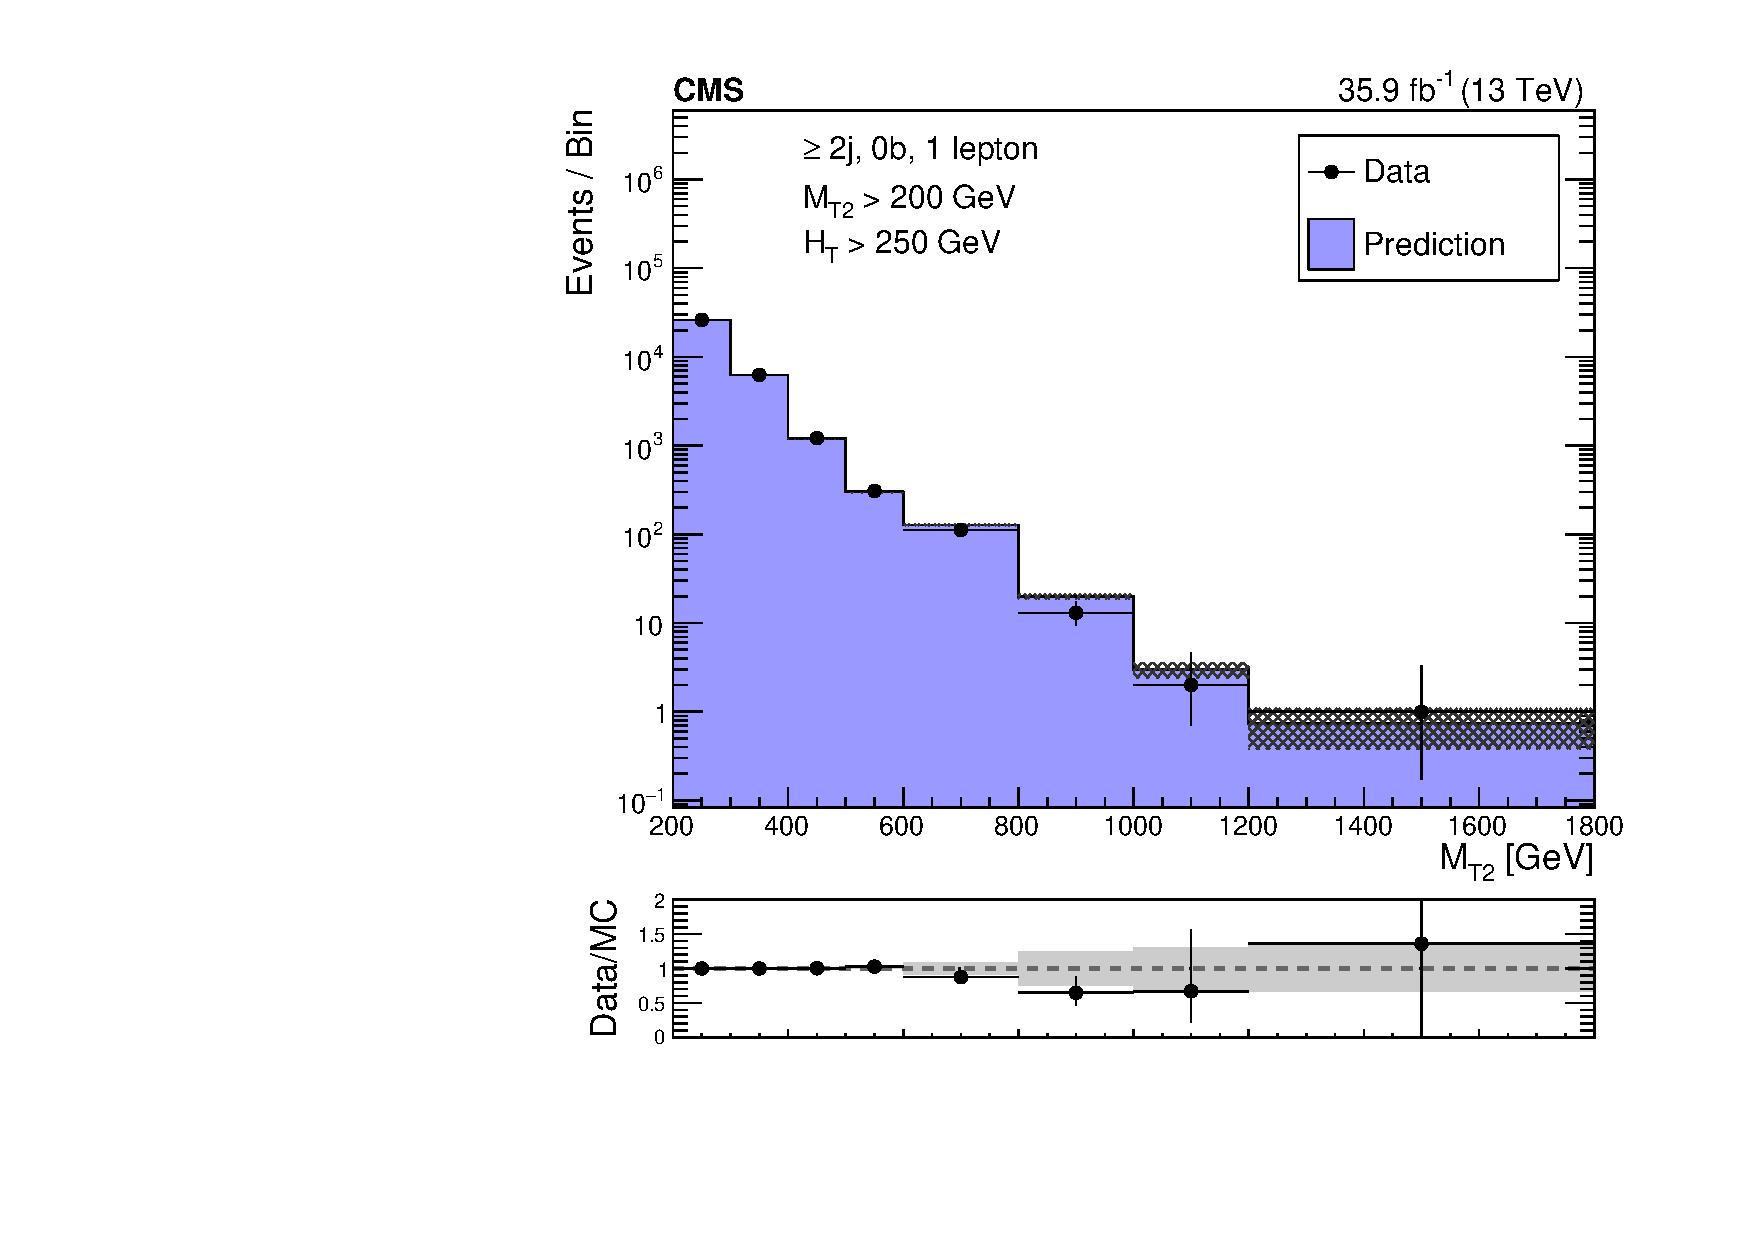
\includegraphics[width=0.45\textwidth]{backgrounds/figs/lostlepHybrid_0b_mt2bins.pdf}
	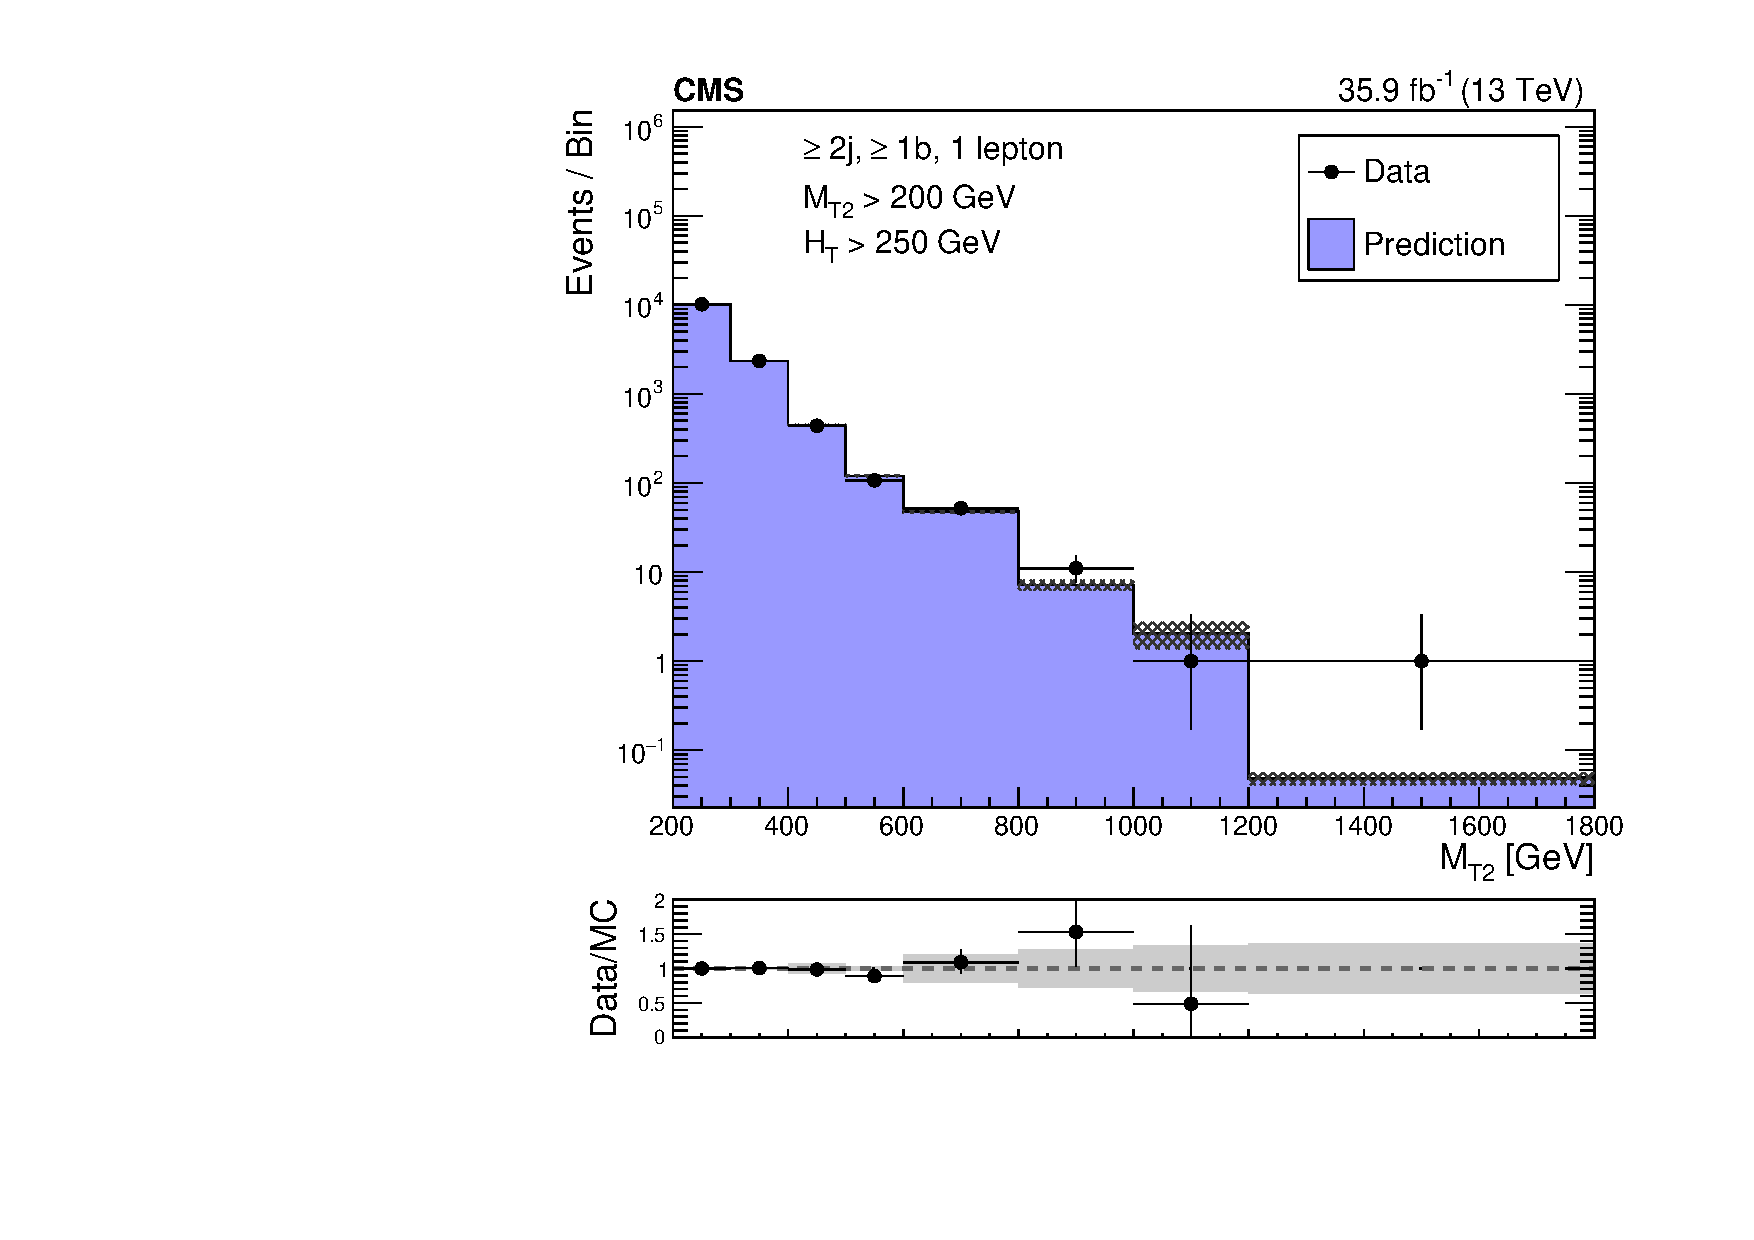
\includegraphics[width=0.45\textwidth]{backgrounds/figs/lostlepHybrid_ge1b_mt2bins}
	\caption{The \mttwo shape in data and simulation using the single lepton CR selection, for events with zero b-tagged jets (left) or at least one b-tagged jet (right). The simulation is normalized to data in each topological region before summing to create the inclusive region. The hatched bands in each upper plot show the MC statistical uncertainty, while the shaded bands in each lower plot represent the systematic shape uncertainty.}
	\label{fig:lostlepHybrid}
\end{figure}

\subsection{Systematic Uncertainties}
\label{subsec:lostlepSyst}

Several sources of uncertainty are assessed for the lost lepton estimate, including those associated with the topological transfer factor and the \mttwo shape modeling in simulation. The full list of systematic uncertainties is as follows:
\begin{itemize}
	\item {\it Control region statistical error:} the Poisson error on the number of observed events in data is taken as a correlated uncertainty in each signal region using the same control region. The error is uncorrelated amongst \mttwo bins, except in regions sharing merged \mttwo bins for the estimate.
	\item {\it Monte Carlo statistical error:} where the simulation is used to compute the transfer factor (and in some cases, the \mttwo shape), the MC statistical uncertainty ranges from 1-50\%, taken as uncorrelated amongst all bins.
	\item {\it Electron and muon selection efficiency:} the reconstruction and identification efficiency of electrons and muons is computed using a procedure known as {\it tag and probe}, where leptons from \Zll decays are used to evaluate the lepton id efficiencies as a function of lepton \pt and $\eta$ and lepton isolation efficiencies as a function of \pt and nearby activity. The scale factors applied to simulation to compensate for such effects approach unity with uncertainties on the order of a few percent, and are correlated across all bins. The maximum effect of this uncertainty is up to 7\% in some signal regions.
	\item {\it Tau selection efficiency:} the efficiency for hadronically decaying taus is classified according to the number of charged particles in the $\tau$ decay, whether a {\it 1-prong} tau leaving a single charged track, or a {\it 3-prong} tau leaving three charged tracks in the final state. This efficiency is measured in simulation by measuring the isolation efficiency as a function of candidate \pt for electrons, muons, and taus in various decay modes. Based on half the difference in efficiency between 1-prong taus and muons, an uncertainty of 10\% is taken for 1-prong taus which also covers and differences in veto efficiency as a function of the primary kinematic variables. For 3-prong taus, the PF hadron veto is very inefficient since most fail the isolation requirement (the typical selection efficiency is 8\%), and a 100\% relative uncertainty is taken to cover any differences as a function of kinematics. These uncertainties are correlated amongst all bins.
	\item {\it \Mt cut efficiency:} the use of simulation to compute the CR-to-SR transfer factor also relies on the satisfactory modeling of the \Mt cut in Monte Carlo. A sample of \Zll events is selected in data with one of the leptons ``deleted'' from the event to mimic a leptonic W boson decay, and compared with simulation. Based on data-MC agreement, a correlated error of 3\% is taken across all bins.
	\item {\it b-tagging efficiency:} the effect of varying the b-tag scale factor efficiency is calculated in each bin, and taken as a correlated error amongst all bins. The maximum effect of this variation is about 4\% in some bins.
	\item {\it Jet energy corrections:} by varying the jet energy scales across all bins, a maximum deviation of about 5\% is observed in regions with sufficient statistics, and a correlated error of 5\% is taken across all bins.
	\item {\it MC renormalization and factorization scales:} the overall effect of varying the simulation renormalization and factorization scales of the underlying physics processes (and subsequent effect on event kinematics) is computed separately in each bin. Taken as correlated across all bins, it is typically on the order of a few percent, but ranges up to 10\% in some regions.
	\item {\it \mttwo shape uncertainty:} in regions where the simulation is used to model the \mttwo distribution, additional variations of the renormalization and factorization scales, parton distribution functions, b-tagging scale factor uncertainties, and jet energy scale uncertainties are performed to measure their effect on the \mttwo shape modeling. The most significant impact is seen in the highest \mttwo bins from theoretical uncertainties ($\sim$15\%), and up to 40\% in low statistics bins due to jet energy scale variations. With this in mind, the shape uncertainty (in regions where MC \mttwo shape modeling is used) is assigned as a linear morphing of the \mttwo shape starting in the first bin from which MC extrapolation is used, growing to 40\% in the final bin. The shape morphing in every distinct topological region is taken as an uncorrelated error.
\end{itemize}


\subsection{Signal Contamination}
\label{subsec:signalContamination}

Nearly every control region in this analysis (including those for multijet and invisible Z backgrounds) is not only orthogonal to the signal region selection, but also crafted such that any potential BSM signal contribution to any CR is negligible and will not bias the background estimate. However, certain SUSY simplified models yield final states with prompt lepton decays --- in some cases kinematically similar to SM \ttbar decays --- which may be non-negligible in the lost lepton CR. To account for this effect when calculating limits on such models (described in detail in section ref{sec:interpretations}), the amount by which the lost lepton background is overestimated is modeled as a loss in signal efficiency. The modified signal yield $N_{\mathrm{sig}}^{SR\prime}$ is defined in equation \ref{eq:signalContamination}, where $N_{\mathrm{sig}}^{SR}$ and $N_{\mathrm{sig}}^{CR}$ represent the simulated signal yield in the signal and control regions respectively, and $TF$ the total transfer factor used in the lost lepton estimate for a given signal region. 
\begin{equation}
	N_{\mathrm{sig}}^{SR\prime} = N_{\mathrm{sig}}^{SR} - TF \cdot N_{\mathrm{sig}}^{CR}
	\label{eq:signalContamination}
\end{equation}
The correction is most significant for simplified models with stop decays, where the stop-neutralino mass splitting is close to the SM top quark mass. In such cases, the signal contamination is maximally 5\% of the expected background yields in each CR for mass points near the expected exclusion limits at high mass.


% --------------------------------------------------------------------------- %
% --------------------------------------------------------------------------- %
